	\section{Object Detection}
	\label{sec:bg:object_detection}
	Object Detection is a well studied topic since the very beginning of computer vision. It can be separated in two individual problems which are Classification: Which object does the image/ a patch of the image contain? and Localization: Where in the image is the object?.
	
	Existing methods can broadly be grouped in three categories. These are described in the following:

	\subsubsection{Shallow Methods}
	
	Usually filters are handcrafted or learned separately. Their response is fed into a classifier. The detector pipeline is applied on the image in sliding window fashion. The results are filtered by a final non-maximum suppression stage. 
	
	Popular features are haar-features \cite{Viola2004} and the Histogram of Gradients\cite{Forsyth}. These methods give good results as long as the object is fully visible and the position in the test set does not change too much. This issue gave raise to deformable part models where parts of the object are modeled individually and connected with mathematical springs \cite{Viola2004}.
	

	\subsubsection{Two Stage Detectors}
	
			\paragraph{Scalable Object Detection using Deep Neural Networks\cite{Erhan}}
			\begin{itemize}
				\item[-] Generates number of bounding boxes as object candidates (class agnostic) and confidences for each box
				\item[-] For each Bounding Box a classifier is run e.g. DNN
				\item[-] Training: If the number of boxes k is larger than the number of objects b, only b boxes are matched while the confidence of the others is minimized
				\item[-] Assignment problem $$F_{match}(x,l) = \frac{1}{2}\sum_{i,j}x_{ij}||l_i - g_j||^2_2$$ where $x_ij$ is one if the ith prediction is assigned to the jth ground truth object
				\item[-] Confidence: 
				$$F_{conf}(x,c) = - \sum_{i,j}x_{ij}*\log(c_i)-\sum_{i}(1-\sum_{j}x_{ij})\log{1-c_j}$$
				\item[-] Speed up training by clustering (kmeans) of ground truth and using it as prior (prior matching)
				\item[-] Can be defined to output boxes only for a particular class by training the bounding boxes on that class
				\item[-] Number of parameters grows linearly with number of classes
				\item[-] Authors argue two step process (region proposal + classification) is better
				\item[-] Architecture based on AlexNet
				\item[-] Predicted boxes are merged using non-maxima surpression
				\item[-] One shot(50\%), +2scales (75\%)
				\item[-] OverFeat/ Selective Search are faster but much more expensive
			\end{itemize}
			
	
	Methods consist usually of two stages.An example is R-CNN\cite{Ren}. 
	\begin{itemize}
		\item Object Proposal: A convolutional net proposes regions that contain an object. This is either done in sliding window fashion or in one pass.
		\item Classification: All proposed regions are fed into a classifier. This can either be a "traditional" one or another CNN.
	\end{itemize}

	\subsubsection{One Stage Detectors}
	
	\begin{figure}[h]
		\centering
		\begin{minipage}{0.4\textwidth}
			\centering
			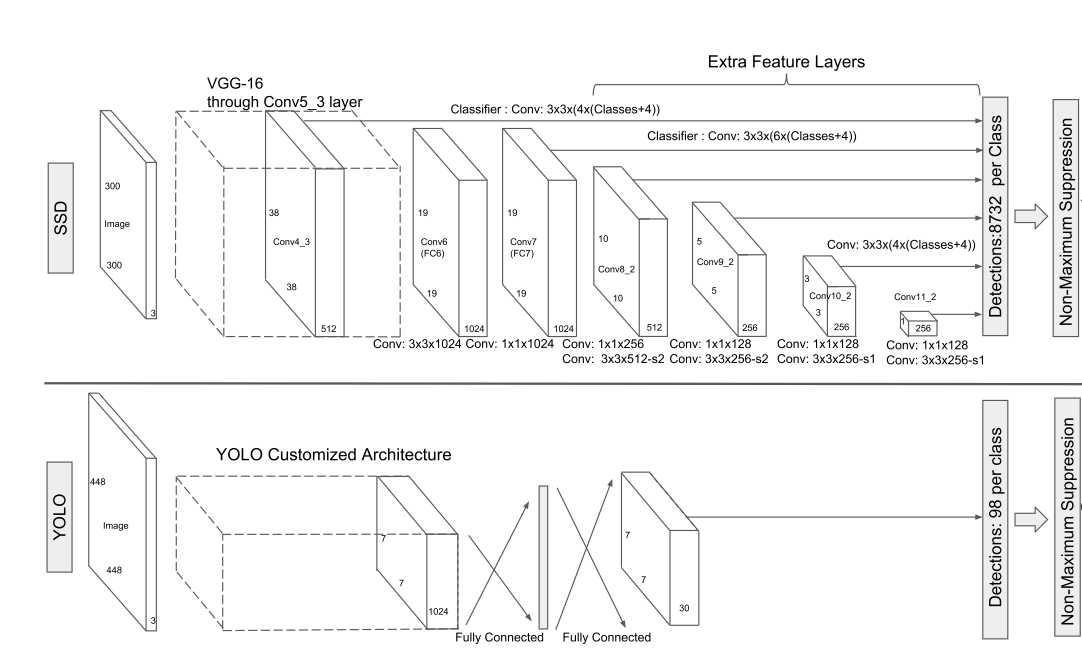
\includegraphics[height=2.5cm]{fig/architecture}
			\caption{Typical Architecture for One Stage Detectors}
			\label{fig:architecture}
		\end{minipage}
		\hspace{2cm}
		\begin{minipage}{0.4\textwidth}
			\centering
			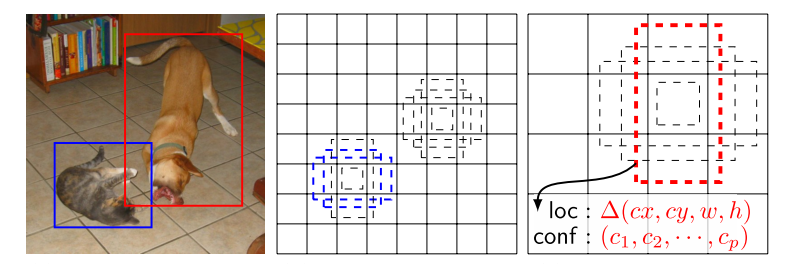
\includegraphics[height=2.5cm]{fig/anchors}
			\caption{Example of \cite{Liu}, the GT box of the cat is matched to two anchor boxes which get responsible for predicting that box. The GT box of the dog is matched to one anchor box.}
			\label{fig:anchors}
		\end{minipage}
	\end{figure}
	
	Most current methods rely on the same principle as Yolo/SSD: A convolutional regression layer is stacked on top of a "base network" that has been trained for image classification e.g. VGG-16. The output layer evaluates feature map(s) of the base network and predicts class confidences, and coordinate offsets for a predetermined set of bounding boxes (so called "prior boxes", "anchor boxes" or "default boxes"). The predictions are filtered in a final non-max-suppression step. During training one has to determine which anchor box is responsible for predicting a certain object. This "matching strategy" differs from method to method but is usually based on the intersection-over-union between the ground truth box and anchor box. \autoref{fig:anchors} illustrates the concept. The final loss function calculates the difference between the responsible boxes and the ground truth. 
	
	Within this framework several approaches exist that either change the base network or modify layers in between: \cite{ChengchengNing2017} propose to include an inception module in the network architecture to reduce computation while keeping/increasing performance. They also propose a more efficient non-max-suppression method. \cite{Wu} uses \textit{SqueezeNet} as base network and a mixture between the ssd and yolo loss function as training goal. \cite{Xiang} investigates the receptive fields of SSD and tries to incorporate more context, especially on lower feature maps, to increase detection rate for small objects.\cite{Linb} applies the framework for vehicle detection. They use \textit{GoogLeNet} as base network (and investigate several others).\cite{TripathiSanDiego} apply a network very similar to YoloV2 and investigate 8bit quantization of the model to make it runnable on embedded devices.
	
	A common problem of one stage detectors is the imbalance between background and object samples. Most methods upweigh the positive samples and/or use hard negative mining. \cite{Lin} introduces the \textit{Focal Loss} which focuses on sparse positive samples by design.
	

	
	\subsection{\cite{Linb}}
	
	\begin{itemize}
		\item Uses GoogLeNet as base network
		\item investigates image augmentation and hard negative mining
		\item Uses confidence score plus class probability although only one object shall be detected
	\end{itemize}
		
	\subsubsection{YoloV3 \cite{Redmona}}
	\begin{itemize}
		\item binary cross entropy loss for class predictions
		\item 3 boxes at each scale (3 scales)
		\item merge lower level features with higher level features and predict another tensor
		\item new network with several residual layers, in between 1x1 convolutions, fully connected layer at the end (53 layers)
		\item runs at 22-51ms depending on resolution
	\end{itemize}

\begin{table}[]
	
	\caption{Object Detection}
	\label{my-label}
	\begin{tabular}{|p{3cm}|p{3cm}|p{3cm}|p{3cm}|p{3cm}|p{3cm}|p{3cm}|p{3cm}|}
		\hline
		& \multicolumn{3}{l|}{Traditional} & \multicolumn{4}{l|}{Deep}   \\ \hline
		& Viola\&Jones    				   & HoG    & DPM   		   & R-CNN    & YOLO         & SSD & OverFeat \\ \hline
		Feature Detector & Haar					   & HoG    & Multiple Hogs and virtual springs   & Learned by CNN     &  Learned by CNN            & & \\ \hline
		Detection & \multicolumn{3}{l|}{Sliding Window, high filter responses indicate there is an object} & NN in sliding window detects regions for possible objects, For each proposed region a classification is run & Image is split in Grid each Grid spawns Bounding boxes and gives class probabilities & & \\
		\hline
		Accuracy (voc) &  & & & 73.2 mAP & 63.4 mAP & 74.3 mAP & \\ 
		\hline
		Speed & & & & 7 FPS (Faster-RCNN) & 45 FPS & 59 FPS & \\
		\hline
		Strengths & & & & & &  &\\
		\hline
		Weaknesses & & & & & &  &\\
		\hline
		\end{tabular}
		
		\end{table}

Each of the described group of methods has strengths and weaknesses. While shallow methods are typically quite fast they require a lot of manual effort and/or are not so accurate. Two-stage detectors on the other hand are quite accurate but their computational requirements are prohibitive for the hardware to be used in this thesis. One-stage detectors offer a compromise between detection accuracy and inference speed. In addition they can be trained end-to-end which requires only little manual engineering. However, the presented methods are still too slow for the hardware used in this thesis.
